
\documentclass[14pt]{beamer}

\mode<presentation>
{
  \usetheme{boxes}
  \usecolortheme[RGB={128,0,0}]{structure}
  \usefonttheme{structurebold}

  \setbeamertemplate{frametitle}[default][center]
  \setbeamertemplate{navigation symbols}{} 
}

\usepackage[english]{babel}
\usepackage[latin1]{inputenc}
\usepackage{times}
\usepackage[T1]{fontenc}
\usepackage{perry-thesis-macros}

\title{Cross-Validation for Principal Components Analysis}

\author[P. O. Perry]{Patrick O. Perry}

\institute[Harvard University]
{
  Statistics and Information Sciences Laboratory\\
  Harvard University
}

\date[BIRS Workshop on Sparse Random Structures]
{January 28, 2010 / BIRS Sparse Random Structures}

\subject{Talks}


\begin{document}

\begin{frame}
  \titlepage
  \hfill\small{(joint work with Art Owen, Stanford)}
\end{frame}


\section{Motivation}
\begin{frame}
  \frametitle{Low-rank matrix approximation}
  \[
    \begin{array}{cccc}
      \mX        & \approx & \mhU       & \mhV^\trans \\
      n \times p &         & n \times k & k \times p
    \end{array}
  \]
  \vskip2em
  \uncover<2->{\centerline{\alert{Problem: How to pick $k$?}}}
\end{frame}

\begin{frame}
  \frametitle{Rank-estimation procedures}
 
  Kritchman \& Nadler survey recently-developed methods
\end{frame}

\begin{frame}
  \frametitle{The data matrix}
  \begin{columns}[c]
  \column{.5\textwidth}
    \[
      \mX
	=
	\left(
	\begin{matrix}
	  \vx_1^\trans \\
	  \vx_2^\trans \\
	  \vdots \\
	  \vx_n^\trans
	\end{matrix}
	\right)
    \]
  \column{.5\textwidth}
    \[
      \vx_{i} \in \reals^p
    \]
  \end{columns}
  \begin{center}
    \begin{itemize}
      \item $n$ and $p$ are both ``big'' \\
      \item $n = \gamma \, p$
    \end{itemize}
  \end{center}
\end{frame}

\begin{frame}
  \frametitle{Truncated SVD}
  \begin{gather*}
    \mX = \sum_{i=1}^{n \wedge p} \sqrt{n} \, \hd_i \vhu_i \vhv_i^\trans = \sqrt{n} \, \mhU \mhD \mhV^\trans \\
    \mhX(k) = \sum_{i=1}^k \sqrt{n} \, \hd_i \vhu_i \vhv_i^\trans = \sqrt{n} \, \mhU \mhD(k) \mhV^\trans
  \end{gather*}

  \begin{itemize}
  \item $\mhD = \diag(\hd_1, \hd_2, \ldots, \hd_{n \wedge p})$
  \item $\mhD(k) = \diag(\hd_1, \hd_2, \ldots, \hd_k, 0, 0, \ldots, 0)$ 
  \end{itemize}
\end{frame}

\begin{frame}
  \frametitle{Signal $+$ noise model}
  \[
    \begin{array}{ccccccc}
      \mX                     &= \sqrt{n} & \mU                        & \mD                          & \mV^\trans   &+ & \mE \\
      \scriptstyle{n\times p} &           & \scriptstyle{n \times k_0} & \scriptstyle{k_0 \times k_0} & \scriptstyle{k_0 \times p} &  & \scriptstyle{n \times p}
    \end{array}
  \]
  \vskip2em
  \begin{itemize}
    \item $\mhU^\trans \mhU = \mhV^\trans \mhV = \mI_{k_0}$ \\
    \item $\mD = \diag(d_1, d_2, \ldots, d_{k_0})$, \, $d_i^2 = \mu_i + \OhP(\frac{1}{\sqrt{n}})$ \\
    \item $\mE_{ij} \sim \Normal(0, \sigma^2)$
  \end{itemize}
\end{frame}

\begin{frame}
  \frametitle{Relation to factor models}
  Standard latent factor model assumes $\vx_i$ i.i.d., \\
  $\cov \vx_1 = \Sigma = \mV \diag(\mu_1, \ldots, \mu_{k_0}) \mV^\trans + \sigma^2 \mI_p$
  
  \vskip2em

  Eigenvalues of $\Sigma$ are: $\mu_1^2 + \sigma^2, \ldots, \mu_{k_0}^2 + \sigma^2,$
  $\sigma^2, \ldots, \sigma^2$.
\end{frame}

\begin{frame}
  \frametitle{Success criterion: model error}
  \[
    \ME(k) \equiv \| \sqrt{n} \mU \mD \mV^\trans - \mhX(k) \|_\Frob^2
  \]
  \begin{itemize}
    \item $\mX = \sqrt{n} \mU \mD \mV^\trans + \mE$
    \item $\mhX(k) = \sqrt{n} \, \mhU \mhD(k) \mhV^\trans$
  \end{itemize}
\end{frame}

\begin{frame}
  \frametitle{Prediction error}
  \[
    \PE(k) \equiv \E \| \mX' - \mhX(k) \|_\Frob^2
  \]
  \begin{itemize}
    \item $\mE' \eqd \mE$
    \item $\mX' = \sqrt{n} \mU \mD \mV^\trans + \mE'$
  \end{itemize}
  \vskip1em
  \[
    \PE(k) = \E\left[ \ME(k) \right] + n p \, \sigma^2
  \]
\end{frame}

\begin{frame}
  \frametitle{Agenda}
  \begin{enumerate}
    \item Analyze behavior of $\ME(k)$, $\PE(k)$
    \item Get estimates $\widehat{\ME}(k)$, $\widehat{\PE}(k)$ via cross-validation
  \end{enumerate}
\end{frame}

\section{Behavior of the SVD}

\subsection{sample singular values and vectors}

\begin{frame}
  \frametitle{Asymptotic behavior of singular values}
  Let $n, p \to \infty$.
  \begin{theorem}[Onatski]
    \[
      \hat d_i^2
      \toas
        \begin{cases}
            \left( \mu_i + \sigma^2 \right)
            \left( 1 + \frac{\sigma^2}{\gamma \mu_i} \right)
                &\text{when $\mu_i > \frac{\sigma^2}{\sqrt{\gamma}}$}, \\
            \sigma^2 \left( 1 + \frac{1}{\sqrt{\gamma}} \right)^2
                &\text{otherwise,}
        \end{cases}
    \]
  \end{theorem} 
\end{frame}

\begin{frame}
  \frametitle{Right singular vectors}
  \begin{theorem}[Onatski, POP]
    \[
      \mV^\trans \mhV(k)
      \toas
      \diag(\theta_1, \theta_2, \ldots, \theta_k)
    \]
    where
    \[
       \theta_i =  \begin{cases}
            \sqrt{ 
                \left( 1 - \frac{\sigma^4}{ \gamma \mu_i^2} \right) 
                \left( 1 + \frac{\sigma^2}{ \gamma \mu_i  } \right)^{-1} }
            &\text{when $\mu_i > \frac{\sigma^2}{\sqrt{\gamma}}$,} \\
            0
            &\text{otherwise,}
        \end{cases} 
    \]
  \end{theorem}
\end{frame}

\begin{frame} 
  \frametitle{Left singular vectors}
  \begin{theorem}[Onatski, POP]
    \[
      \mU^\trans \mhU(k)
      \toas
      \diag(\varphi_1, \varphi_2, \ldots, \varphi_k)
    \]
    where
    \[
      \varphi_i =
        \begin{cases}
            \sqrt{
                \left( 1 - \frac{\sigma^4}{ \gamma \mu_i^2} \right)
                \left( 1 + \frac{\sigma^2}{ \mu_i  } \right)^{-1} }
            &\text{when $\mu_i > \frac{\sigma^2}{\sqrt{\gamma}}$,} \\
            0
            &\text{otherwise,}
        \end{cases}
    \]
  \end{theorem}
\end{frame}

\subsection{loss behavior}

\begin{frame}
  \frametitle{Model error}
  \begin{theorem}
\begin{equation*}
    p \cdot {\ME} (k)
        \toas
        \sum_{i=1}^{k}
            \alpha_i \mu_i
        +
        \sum_{i=k+1}^{k_0}
            \mu_i
        +
        \sigma^2
        \left(
            1 + \frac{1}{\sqrt{\gamma}}
        \right)^2
        \cdot
        (k - k_0)_+,
\end{equation*}
where
\begin{equation*}
    \alpha_i 
    =
    \begin{cases}
        \frac{\sigma^2}{\gamma \mu_i^2}
                \big(
                    3 \sigma^2 + (\gamma+1) \mu_i
                \big)
            &\text{if $\mu_i > \frac{\sigma^2}{\sqrt{\gamma}}$,} \\
        1 
        + 
        \frac{\sigma^2}{\mu_i}
        \left(
            1
            +
            \frac{1}{\sqrt{\gamma}}
        \right)^2
            &\text{otherwise.}
    \end{cases}
\end{equation*}
\end{theorem}
\end{frame}

\begin{frame}
  \frametitle{Frobenius penalty for including $i$th term}
  \begin{center}
  \includegraphics[scale=0.6]{frobenius-loss-penalty}
  \end{center}
\end{frame}

\begin{frame}
  \frametitle{Threshold for inclusion}
  only beneficial to include $i$th term when $\mu_i$ above threshold
  \begin{center}
  \includegraphics[scale=0.6]{frobenius-loss-cutoff}
  \end{center}
\end{frame}
\subsection{simulations}

\begin{frame}
  \frametitle{Simulation}
  \begin{itemize}
  \item $\gamma = \frac{n}{p} \in \{ 0.25, 1.0, 4.0 \}$
  \item size $n p \in \{ 144, 400, 1600, 4900 \}$
  \item $k_0 = 5$
  \item two components above threshold, two below (one equal)
  \end{itemize}
\end{frame}

\begin{frame}
  \frametitle{Results}
  \begin{center}
  \includegraphics[scale=0.6]{frob2-loss-sim}
  \end{center}
\end{frame}


\section{Cross-validation}

\begin{frame}
  \frametitle{Cross-validation}
  \textbf{use cross-validation (CV) to estimate $\ME(k)$}
  \begin{enumerate}
  \item partition data into \textsc{train} (holdin) and \textsc{test} (holdout) set
  \item fit model to \textsc{train} set   
  \item evaluate performance of model on \textsc{test} set
  \item repeat over many partitions of the data
  \end{enumerate}
\end{frame}

\subsection{Wold-style holdouts}

\begin{frame}
  \frametitle{Wold-style ``speckled'' holdouts}
  \begin{enumerate}
    \item hold out a random subset of elements of $\mX$
    \item fit SVD using expectation-maximizaiton (EM)
    \item evaluate performance
  \end{enumerate}
\end{frame}

\subsection{Gabriel-style holdouts}

\begin{frame}
  \frametitle{Gabriel-style ``blocked'' holdouts}
  \begin{enumerate}
    \item partition
    \(
      \mX = \left(\begin{matrix} \mX_{11} & \mX_{12} \\ \mX_{21} & \ast \end{matrix}\right)
    \)
    \item $\mhU_1 \mhD_1 \mhV_1^\trans$ is the SVD of $\mX_{11}$
    \item $\mhX_{22}(k) = \mX_{21} \mhV_1 \mhD_1(k)^+ \mhU_1^\trans \mX_{12}$ is the prediction of the holdout set
  \end{enumerate}
\end{frame}

\begin{frame}
  \frametitle{Rotated versions}
  Replace $X$ with $\mO_L^\trans \mX \mO_R$, for random orthogonal $\mO_\cdot$. 
\end{frame}

\begin{frame}
  \frametitle{Simulations}
  \begin{itemize}
    \item factors $\mU$ and $\mV$ are either ``Gaussian'' or ``sparse''
    \item signal strength $\mD$ is either ``strong'' or ``weak''
    \item black is true model error
    \item red is CV estimate
    \item blue is rotated-CV estimate
  \end{itemize}
\end{frame}

\begin{frame}
  \frametitle{Strong Gaussian factors}
  \begin{center}
  \includegraphics[scale=0.55]{cvsvd-strong-gauss}
  \end{center}
\end{frame}

\begin{frame}
  \frametitle{Strong sparse factors}
  \begin{center}
  \includegraphics[scale=0.55]{cvsvd-strong-sparse}
  \end{center}
\end{frame}
\subsection{theory}

\begin{frame}
  \frametitle{Weak Gaussian factors}
  \begin{center}
  \includegraphics[scale=0.55]{cvsvd-weak-gauss}
  \end{center}
\end{frame}


\begin{frame}
  \frametitle{Weak sparse factors}
  \begin{center}
  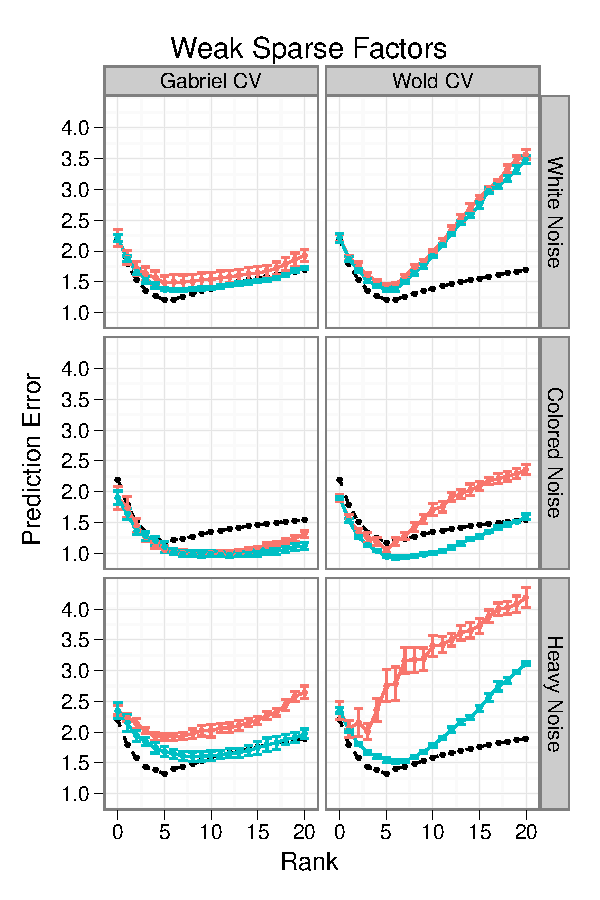
\includegraphics[scale=0.55]{cvsvd-weak-sparse}
  \end{center}
\end{frame}

\begin{frame}
  \frametitle{Theory for Gabriel-style}
  \begin{itemize}
  %\item $\hat \sigma^2$ is a $\sqrt{np}$ consistent estimator of $\sigma^2$
  \item technical assumption on factor sparsity
  \end{itemize}
  \begin{theorem}
  \[
\E \left[ p \cdot \widehat{\ME}_n(k) \right]
			\to
				\sum_{i=1}^{k \wedge k_0}
					\beta_i \, \mu_i
				+
				\sum_{i=k+1}^{k_0}
					\mu_i
				+
				\eta
				\cdot
				(k - k_0)_+,
  \]
  where $\beta_i = \ldots$, $\eta_i = \ldots$
  \end{theorem}
\end{frame}

\begin{frame}
  \frametitle{Optimal leave-out size}
  By comparing $\alpha_i$ and $\beta_i$, we determine the optimal leave-out size.
  \begin{theorem}
    If
    \[
       \sqrt{\frac{n_1 p_1}{n p}}
       =
       \frac{\sqrt{2}}{\sqrt{\bar \gamma} + \sqrt{\bar \gamma + 3}}
    \]
    then minimizer of $\E\left[\widehat{ME}(k)\right]$ is same as minimizer of $\ME(k)$;
    here
    \(
      \bar \gamma = (\gamma^{1/2} + \gamma^{-1/2})^2/4
    \),
    $\mX_{11}$ is $n_1 \times p_1$
  \end{theorem}
\end{frame}

\begin{frame}
  \frametitle{What else?}
  \begin{itemize}
    \item scree plot
    \item benchmark with other rank-selection algorithms
    \item intuition behind Gabriel-style (blocked) leave-outs
    \item proofs of results
    \item applications to real data
  \end{itemize}
\end{frame}

\begin{frame}
  \frametitle{Open problems}
  \begin{itemize}
    \item theory for Wold-style leave-outs
    \item which is better: Wold-style or Gabriel-style?
    \item theory for other low-rank decompositions
  \end{itemize}
\end{frame}

\begin{frame}
  \frametitle{References}
  \begin{itemize}
    \item Owen \& Perry. Annals of Applied Statistics. 2009
    \item Perry. PhD Thesis, ``Cross-Validation for Unsupervised Learning.''
      2009.
    \item both at \texttt{ptrckprry.com/reports}
  \end{itemize}
\end{frame}

\begin{frame}
  \frametitle{R package}
  \texttt{bcv} (``Bi-cross-validation'') available on CRAN
\end{frame}

\begin{frame}
  \centerline{Thank you!}
\end{frame}

\end{document}


